\documentclass{report}
\usepackage[spanish]{babel}
\usepackage[left=2.5cm, right=2.5cm, top=3cm, bottom=3cm]{geometry}
\usepackage{enumerate}
\usepackage{graphicx}
\usepackage{booktabs}
\usepackage{tabularx}
\usepackage{enumitem}
\usepackage{amsmath}
\usepackage{amsfonts}
\usepackage{float}
\usepackage{hyperref}   



\setlength{\parindent}{0pt}

\begin{document}

    \begin{titlepage}
        \centering
        {\bfseries\LARGE Facultad de Matemática y Computación \par}
        \vspace*{1cm}
        {\scshape\Large Ingeniería de Software \par}
        \vspace*{3cm}
        {\scshape\Huge Informe de Especificación de Requerimientos \par}
        \vspace*{1cm}
        {\LARGE \textbf{Tema: Gestión de campeonatos de béisbol} }
        \vfill
        {\bfseries\LARGE Integrantes: \par}
        {\Large Ariadna Vel\'azquez Rey  C311 \par} 
        {\Large L\'ia L\'opez Rosales  C312 \par} 
        {\Large Carlos Daniel Largacha Leal  C312 \par} 
        {\Large Gabriel Andr\'es Pla Lasa  C311 \par} 
        {\Large Raidel Miguel Cabellud Lizaso C311 \par} 
        \vfill
    \end{titlepage}

    \begin{center}
        \section*{Introducción}
    \end{center}

        \subsection*{Propósito del Documento}
        El propósito de este documento es definir y detallar los requerimientos del sistema de gestión de campeonatos de béisbol. Su objetivo principal es servir como una referencia clara y precisa para los desarrolladores, diseñadores y demás partes interesadas en el proyecto, asegurando que la aplicación cumpla con las necesidades de los usuarios. 

        Proporciona una visión integral del sistema, abarcando su alcance, funcionalidades, restricciones y requisitos técnicos. Además, establece las bases para futuras mejoras y mantenibilidad, garantizando una implementación eficiente y alineada con las expectativas del cliente y los usuarios finales.


        \subsection*{Alcance del Producto}

        Este proyecto tiene como objetivo el desarrollo de una aplicación web que facilite la gestión de los 
        campeonatos de béisbol. Su propósito principal es permitir a los usuarios consultar y analizar información 
        relevante de las series y los peloteros, proporcionando herramientas que soporten la toma de decisiones 
        basada en estadísticas detalladas y actualizadas. El sistema será accesible, eficiente y adaptado a las 
        necesidades de diversos usuarios, desde administradores hasta periodistas.


        \subsection*{Definiciones, acrónimos y abreviaturas}
        \textbf{PDF(Portable Document Format):} Es un formato de almacenamiento para documentos 
        digitales independientes de plataformas de software o hardware.

        \subsection*{Resumen del resto del documento}
        El presente documento se estructura en varias secciones clave:

        \begin{itemize}
            \item \textbf{Descripción General:} Se proporciona una visión global del sistema, incluyendo su propósito, alcance y los actores involucrados.
            \item \textbf{Requerimientos Funcionales:} Se detallan las funciones esenciales del sistema.
            \item \textbf{Requerimientos No Funcionales:} Se especifican criterios como usabilidad, seguridad, escalabilidad y compatibilidad que el sistema debe cumplir.
            \item \textbf{Requerimientos de Entorno:} Se definen los aspectos técnicos necesarios para el correcto funcionamiento del software, incluyendo hardware, software y bases de datos.
            \item \textbf{Anexos:} Se incluyen diagramas y material adicional que complementan la especificación de requerimientos.
        \end{itemize}

    \newpage

    \begin{center}
        \section*{Descripción General}
    \end{center}

        \subsection*{Perspectiva del Producto}
        La aplicación web será una solución integral para la gestión y consulta de estadísticas en campeonatos de 
        béisbol. Estará diseñada para ofrecer:
        \begin{itemize}
            \item Una landing pública de acceso libre, sin necesidad de autenticación.
            \item Acceso a estadísticas detalladas de series, equipos y jugadores.
            \item Generación de reportes personalizados con exportación a PDF/CSV.
            \item Funcionalidades diferenciadas según el rol del usuario (administrador, director técnico, 
            periodista/usuarios generales, invitados, etc.).
            \item Servicios personalizados para usuarios con cuenta: favoritos, notificaciones y panel personal.
            \item Perfiles detallados de equipos y jugadores, y comparador de peloteros.
        \end{itemize}

        \subsection*{Funciones del Producto}
        
        \begin{enumerate}
        \item \textbf{Descripción de los Actores}

            \begin{itemize}
                \item \textbf{Administrador:} Responsable de gestionar los datos de series, equipos y jugadores, 
                además de configurar el sistema y generar reportes.
                \item \textbf{Director Técnico:} Encargado de gestionar las alineaciones de los equipos y consultar 
                estadísticas específicas.
                \item \textbf{Periodista/Usuario General:} Consulta las estadísticas y genera reportes basados en 
                los datos almacenados en el sistema.
                \item \textbf{Invitado:} Visitante sin sesión. Consulta la información pública (landing, consultas,
                reportes y perfiles) pero no puede exportar ni usar los servicios personalizados.
            \end{itemize}

        \item \textbf{Casos de Uso del Sistema} (que se muestran ilustrados en la Figura 1)
            
            \subsubsection{Registrar datos en el sistema}
            \begin{itemize}
                \item \textbf{Actor:} Administrador
                \item \textbf{Descripción:} El administrador registra datos de series, equipos y jugadores mediante 
                formularios en la aplicación web.
            \end{itemize}

            \subsubsection{Gestionar alineaciones de equipos}
            \begin{itemize}
                \item \textbf{Actor:} Director Técnico y Administrador
                \item \textbf{Descripción:} Permite al director técnico modificar la posición de los jugadores en 
                la alineación inicial y realizar ajustes durante una serie.
            \end{itemize}

            \subsubsection{Consultar estadísticas de jugadores y equipos}
            \begin{itemize}
                \item \textbf{Actor:} Administrador, Director Técnico, Periodista/Usuario General
                \item \textbf{Descripción:} El sistema permite acceder a estadísticas detalladas, como promedios de 
                bateo, efectividad de los lanzadores y resultados de los equipos.
            \end{itemize}

            \subsubsection{Obtener reportes personalizados}
            \begin{itemize}
                \item \textbf{Actor:} Administrador, Director Técnico, Periodista/Usuario General
                \item \textbf{Descripción:} Genera reportes en formato PDF o gráficos que resumen el desempeño de 
                jugadores y equipos en una serie.
            \end{itemize}

            \subsubsection{Visualizar datos tabulares y gráficos}
            \begin{itemize}
                \item \textbf{Actor:} Administrador, Director Técnico, Periodista/Usuario General
                \item \textbf{Descripción:} Presentación visual de estadísticas mediante tablas y gráficos para un 
                análisis claro y rápido.
            \end{itemize}

            \subsubsection{Listar equipos por clasificación}
            \begin{itemize}
                \item \textbf{Actor:} Administrador, Director Técnico, Periodista/Usuario General
                \item \textbf{Descripción:} Permite obtener la clasificación de los equipos según los resultados de 
                cada serie.
            \end{itemize}

            \subsubsection{Modificar roles de usuarios}
            \begin{itemize}
                \item \textbf{Actor:} Administrador
                \item \textbf{Descripción:} El administrador puede asignar o modificar roles para los usuarios del 
                sistema.
            \end{itemize}

            \subsubsection{Exportar reportes a formato PDF}
            \begin{itemize}
                \item \textbf{Actor:} Administrador, Director Técnico, Periodista/Usuario General
                \item \textbf{Descripción:} Funcionalidad para guardar reportes generados en formato PDF, con 
                soporte para otros formatos adicionales.
            \end{itemize}

        \end{enumerate}


        \subsection*{Características de los usuarios}
        El sistema contará con diferentes perfiles de usuarios:
        \begin{itemize}
            \item \textbf{Invitados}: Visualizan toda la información pública del sitio (estadísticas,
            consultas, reportes y perfiles) sin necesidad de registrarse.
            \item \textbf{Administradores}: Control total del sistema, incluyendo la estructura de las series.
            \item \textbf{Directores Técnicos}: Gestión de alineaciones y rendimiento de los equipos.
            \item \textbf{Periodistas/Usuarios Generales}: Consulta de información general sobre los campeonatos. 
            Acceso a estadísticas y reportes para análisis independiente.
        \end{itemize}


        \subsection*{Restricciones generales}
        \begin{itemize}
            \item \textbf{Accesibilidad}: La aplicación será multiplataforma, garantizando su uso desde dispositivos 
            móviles y de escritorio.
            \item \textbf{Disponibilidad}: Asegurará el acceso continuo a la información para usuarios autorizados.
            \item \textbf{Tecnologías}: El desarrollo empleará Django como ORM, bajo una arquitectura hibrida de 
            N-Capas con Microkernel, siguiendo la metodología DIC.
            \item \textbf{Seguridad}: Se implementarán mecanismos para proteger la confidencialidad, integridad y 
            disponibilidad de los datos.
        \end{itemize}

        \subsection*{Dependencias y suposiciones}
        El software no estará sujeto a ningún SO pues se podrá acceder a él a través de cualquier navegador web que 
        el usuario posea.
        
        El lenguaje a utilizar será técnico referente al béisbol pues los usuarios están acontumbrados a él y es 
        necesario para un correcto manejo de los datos guardados.

    \newpage
    
    \begin{center}
        \section*{Requerimientos Específicos}
    \end{center}

    \vspace{0.5cm}

        \subsection*{Requerimientos Funcionales}
            \begin{enumerate}
                \item Mostrar una \textbf{landing pública} con el estado del campeonato: resumen ejecutivo,
                tabla de posiciones, líderes de bateo, jugadores estrella, campeones por temporada y líder
                de la temporada.
                \item Ofrecer \textbf{dos temas visuales} (oscuro y claro) persistidos en el navegador y
                accesibles desde toda la aplicación.
                \item Permitir el \textbf{registro público}: un visitante crea su cuenta (nombre, apellido,
                correo y contraseña) obteniendo automáticamente el rol de Usuario General.
                \item Permitir \textbf{iniciar y cerrar sesión} (token de autenticación) con vistas
                diferenciadas según el rol.
                \item Registrar, editar, eliminar y listar datos por el administrador mediante formularios
                dinámicos (\textbf{Panel Administrativo CRUD} de las entidades del sistema).
                \item Listar y filtrar según sus categorías definidas, nombres de equipos ganadores y
                directores técnicos en series nacionales por temporada.
                \item Listar y filtrar según sus categorías definidas, nombres y posiciones de jugadores del
                equipo "Todos Estrellas" y su rendimiento por serie.
                \item Listar y filtrar según sus categorías definidas, series con mayor y menor cantidad de
                juegos celebrados.
                \item Listar equipos en primer y último lugar por serie, clasificados por tipo y orden
                cronológico.
                \item Listar y filtrar según sus categorías definidas, total de juegos ganados por un
                lanzador y su promedio de carreras limpias permitidas.
                \item Listar y filtrar según sus categorías definidas, estadísticas de un jugador.
                \item Ofrecer \textbf{consultas dinámicas} sobre las entidades del sistema con listado y
                filtros por texto, número o fecha.
                \item Mostrar \textbf{reportes oficiales} preseccionando el primer parámetro disponible
                (temporada, serie o equipo) para que ningún reporte quede vacío.
                \item Exportar reportes a formato \textbf{PDF} y \textbf{CSV} con la identidad visual de la
                LNB, restringido a usuarios autenticados.
                \item Permitir \textbf{imprimir la boleta técnica} con el corte completo de registros y
                descargar el boletín técnico en PDF con la marca del reporte actual.
                \item Mostrar el \textbf{perfil de equipo}: ficha de franquicia, récord con split
                local/visitante, KPIs colectivos, rankings, campeonatos por serie, distribución del plantel,
                próximos juegos y desglose de la temporada, con descarga del roster oficial en PDF.
                \item Mostrar el \textbf{perfil de jugador}: datos personales, estadísticas de bateo y
                pitcheo, radar de rendimiento de 6 ejes y trayectoria reciente en las últimas series.
                \item Ofrecer un \textbf{comparador de peloteros} lado a lado (solo usuarios con cuenta).
                \item Permitir \textbf{marcar favoritos} de equipos y jugadores y listarlos en la landing,
                con un panel personal ("Tu panel") que muestra posición del equipo favorito, últimos juegos
                y estrella del equipo (solo usuarios con cuenta).
                \item Generar \textbf{notificaciones automáticas} al registrar un resultado para los
                seguidores de ambos equipos, con contador de no leídas, marcado individual o global y
                actualización periódica (solo usuarios con cuenta).
                \item Proporcionar al \textbf{Director Técnico} un portal de cambios con lineup titular
                WBSC, diamante defensivo, bullpen filtrable por posición, métricas del equipo y validación
                de juegos futuros en backend.
                \item Mostrar el \textbf{historial de cambios} del Director Técnico con ordenamiento,
                paginación, alta y baja de cambios.
                \item Presentar diferentes vistas para los distintos tipos de roles, bloqueando los accesos
                insuficientes con una pantalla de acceso denegado.
            \end{enumerate}

        \vspace{1cm}

        \subsection*{Requerimientos No Funcionales}

            \vspace{0.3cm}

            \subsubsection*{Usabilidad}
            \begin{itemize}
                \item Se espera que la interfaz sea capaz de mostrar gráficas y diagramas (barras y radar).
                \item Se espera un sistema visual de filtrado para seleccionar qué datos mostrar en los reportes.
                \item La interfaz debe cumplir los criterios de contraste de accesibilidad WCAG AA en ambos temas.
            \end{itemize}
        
            \subsubsection*{Seguridad}
            \begin{itemize}
                \item Todos los datos personales y críticos deben ser encriptados en tránsito y en almacenamiento.
                \item La autenticación y autorización deben ser seguras, permitiendo que solo los usuarios 
                autorizados tengan acceso a funcionalidades específicas.
            \end{itemize}
        
            \subsubsection*{Portabilidad y Compatibilidad}
            \begin{itemize}
                \item El diseño de la interfaz se espera que sea ajustable al tamaño de los distintos dispositivos 
                en los que puede abrirse el sitio web.
                \item Debe ser compatible con los navegadores más utilizados, asegurando que las interfaces web 
                sean responsivas y adaptativas.
            \end{itemize}
        
            \subsubsection*{Rendimiento}
            \begin{itemize}
                \item El sistema debe ser capaz de manejar múltiples solicitudes simultáneamente sin una degradación 
                significativa en el tiempo de respuesta.
            \end{itemize}
        
            \subsubsection*{Escalabilidad}
            \begin{itemize}
                \item La arquitectura debe permitir la escalabilidad horizontal y vertical. Esto significa que se 
                debe poder agregar más recursos (como servidores adicionales) para manejar un mayor número de 
                usuarios o datos sin necesidad de reestructurar significativamente el sistema.
            \end{itemize}
        
            \subsubsection*{Mantenibilidad}
            \begin{itemize}
                \item El sistema debe estar desarrollado con buenas prácticas de programación, como la documentación 
                adecuada (docstring) y código modular.
            \end{itemize}
        
            \subsubsection*{Extensibilidad}
            \begin{itemize}
                \item La arquitectura del sistema debe ser flexible para permitir la adición de nuevas funcionalidades 
                sin necesidad de grandes modificaciones en el código base.
            \end{itemize}
        
            \subsubsection*{Almacenamiento, importación y exportación de datos}
            \begin{itemize}
                \item El software deberá de almacenar todos los datos en una base de datos SQL.
                \item El software deberá ser capaz de convertir los reportes solicitados a documentos PDF.
            \end{itemize}

        \vspace{1cm}

        \subsection*{Requerimientos de Entorno}

            Para garantizar la ejecución del sistema, se deben cumplir las siguientes condiciones:

            \subsubsection{Hardware}
            \begin{itemize}
                \item Dispositivos capaces de ejecutar navegadores modernos y conexiones a internet estables.
                \item En producción, un plan gratuito de Render (backend 512~MB) + una base de datos
                serverless de Neon.
            \end{itemize}
            
            \subsubsection{Software}
            \begin{itemize}
                \item Para la base de datos se ha de utilizar la tecnología PostgreSQL.
                \item En cuanto al backend de la aplicación web, este de desarrollará en Python con DjangoRest como 
                librería principal, omitiendo la función de admin que viene ya preparada.
                \item El frontend se realizará en JavaScript con el framework de React.
                \item Los reportes y las fichas PDF se generan con la librería reportlab.
            \end{itemize}

    \newpage

    \section*{Anexos}

    \begin{figure}[H]
        \centering
        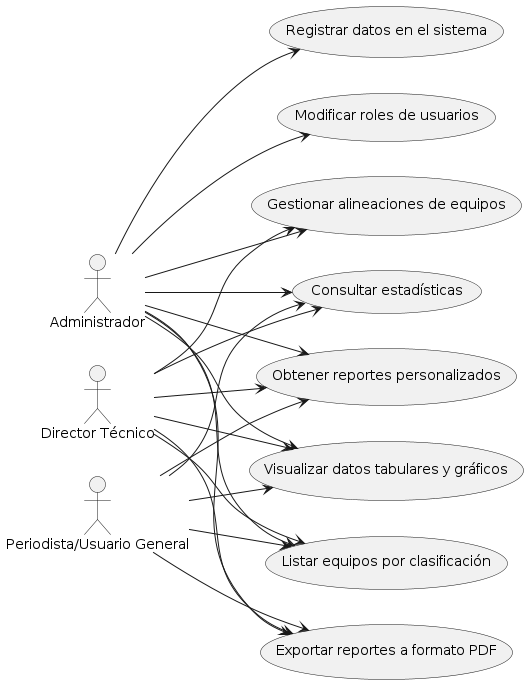
\includegraphics[scale=0.9,keepaspectratio]{caso_de_uso.png}
        \caption{Diagrama de casos de uso}
    \end{figure}


\end{document}